\documentclass{ctexbook}
\usepackage{xeCJK}
\usepackage{amsmath}
\usepackage{titlesec}

\usepackage{enumitem}
\renewcommand\labelenumi{(\theenumi)}

\usepackage{scrextend}% not needed with a KOMA-Script class, provides the
                      % `addmargin' environment

\usepackage{exsheets}
\DeclareInstance{exsheets-heading}{mylist}{default}{
  runin = true ,
  attach = {
    main[l,vc]number[l,vc](-3em,0pt) ; % 3em = indent of question body
    main[r,vc]points[l,vc](\linewidth+\marginparsep,0pt)
  }
}
\SetupExSheets{
  headings = mylist , % use the new headings instance
  headings-format = \normalfont ,
  %counter-format = \thechapter.qu ,
  counter-within = section ,
  solution/print = true
}
\let\oldquestion\question
\let\oldsolution\solution

\renewenvironment{question}{%
	\SetupExSheets{counter-format=\thechapter.qu}
	\oldquestion
}

\renewenvironment{solution}{%
	\SetupExSheets{counter-format=}
	\oldsolution
}

\usepackage{etoolbox}
% 3em = indent of question body :
\AtBeginEnvironment{question}{\addmargin[3em]{0em}}
\AtEndEnvironment{question}{\endaddmargin}
\AtBeginEnvironment{solution}{\addmargin[3em]{0em}}
\AtEndEnvironment{solution}{\endaddmargin}

\title{人工智能及其应用(第4版)\\ 习题解析}
\date{}

\begin{document}
\maketitle

\chapter{绪论}

\begin{question}
什么是人工智能?试从学科和能力两方面加以说明。
\end{question}	
\begin{solution}
人工智能(学科):人工智能(学科)是计算机科学中涉及研究、设计和应用智能机器的一个分支。其近期主要目标在于研究用机器来模仿和执行人脑的某些智力功能,并开发相关理论和技术。\par
人工智能(能力):人工智能(能力)是智能机器所执行的通常与人类智能有关的智能行为,这些智能行为涉及学习、感知、思考、理解、识别、判断、推理、证明、通信、设计、规划、行动和问题求解等活动。
\end{solution}

\begin{question}
在人工智能的发展过程中,有哪些思想和思潮起了重要作用?
\end{question}
\begin{solution}
控制论之父维纳1940年主张计算机五原则。他开始考虑计算机如何能像大脑一样工作。系统地创建了控制论,根据这一理论,一个机械系统完全能进行运算和记忆。\par
帕梅拉·麦考达克(Pamela McCorduck)在她的著名的人工智能历史研究《机器思维》(\textit{Machine Who Think}, 1979)中曾经指出:在复杂的机械装置与智能之间存在着长期的联系。\par
著名的英国科学家图灵被称为人工智能之父,图灵不仅创造了一个简单的通用的非数字计算模型,而且直接证明了计算机可能以某种被理解为智能的方法工作。提出了著名的图灵测试。\par
数理逻辑从19世纪末起就获迅速发展;到20世纪30年代开始用于描述智能行为。计算机出现后,又在计算机上实现了逻辑演绎系统。\par
1943年由生理学家麦卡洛克(McCulloch)和数理逻辑学家皮茨(Pitts)创立的脑模型,即MP模型。60-70年代,联结主义,尤其是对以感知机(perceptron)为代表的脑模型的研究曾出现过热潮。\par
控制论思想早在40-50年代就成为时代思潮的重要部分,影响了早期的人工智能工作者。到60-70年代,控制论系统的研究取得一定进展,播下智能控制和智能机器人的种子。 
\end{solution}

\begin{question}
在过去的20年中,人工智能发生了什么变化?
\end{question}
\begin{solution}
\end{solution}

\begin{question}
为什么能够用机器(计算机)模仿人的智能?
\end{question}
\begin{solution}
物理符号系统假设:任何一个系统,如果它能够表现出智能,那么它就必定能够执行输入符号、输出符号、存储符号、复制符号、建立符号结构、条件性迁移6种功能。反之,任何系统如果具有这6种功能,那么它就能够表现出智能;这种智能指的是人类所具有的那种智能。\par
物理符号系统的假设伴随有3个推论:\par
	\begin{enumerate}
		\item 既然人具有智能,那么他(她)就一定是个物理符号系统。
		\item 既然计算机是一个物理符号系统,它就一定能够表现出智能。
		\item 既然人是一个物理符号系统,计算机也是一个物理符号系统,那么我们就能够用计算机来模拟人的活动。
	\end{enumerate} \par
因此,计算机可以模拟人的智能。
\end{solution}

\begin{question}
现在人工智能有哪些学派?它们的认知观是什么?现在这些学派的关系如何?
\end{question}
\begin{solution}
符号主义(Symbolicism),又称为逻辑主义(Logicism)、心理学派(Psychlogism)或计算机学派(Computerism),认为人工智能源于数理逻辑。 其原理主要为物理符号系统(即符号操作系统)假设和有限合理性原理。符号主义认为人的认知基元是符号,而且认知过程即符号操作过程。它认为人是一个物理符号系统,计算机也是一个物理符号系统,因此,我们就能够用计算机来模拟人的智能行为。它还认为,知识是信息的一种形式,是构成智能的基础。人工智能的核心问题是知识表示、知识推理和知识运用。 符号主义认为人工智能的研究方法应为功能模拟方法。通过分析人类认知系统所具备的功能和技能,然后用计算机模拟这些功能,实现人工智能。\par
连接主义(Connectionism),又称为仿生学派(Bionicsism)或生理学派(Physiologism) ,认为人工智能源于仿生学,特别是人脑模型的研究。其原理主要为神经网络及神经网络间的连接机制与学习算法。连接主义认为人的思维基元是神经元,而不是符号处理过程。认为人脑不同于电脑,并提出联结主义的大脑工作模式,用于取代符号操作的电脑工作模式。 连接主义主张人工智能应着重于结构模拟,即模拟人的胜利神经网络结构,并认为功能、结构和智能行为是密切相关的。不同的结构表现出不同的功能和行为。\par
行为主义(Actionism),又称进化主义(Evolutionism)或控制论学派(Cyberneticsism), 认为人工智能源于控制论。其原理为控制论及感知-动作型控制系统 。行为主义认为智能取决于感知和行动,提出智能行为的“感知-动作”模式。认为智能不需要知识、不需要表示、不需要推理;人工智能可以像人类智能一样逐步进化。智能行为只能在现实世界中与周围环境交互作用而表现出来。行为主义还认为:符号主义、联结主义对真实世界客观事物的描述及其智能行为工作模式是过于简化的抽象,因而是不能真实地反映客观存在的。 行为主义认为人工智能的研究方法应采用行为模拟方法,也认为功能、结构和智能行为是不可分的。不同行为表现出不同功能和不同控制结构。
\end{solution}

\begin{question}
你认为应从哪些层次对认知行为进行研究?
\end{question}
\begin{solution}
人的认知活动具有不同的层次,对认知行为的研究也应具有不同的层次,以便不同学科之间分工协作,联合攻关,早日解开人类认知本质之谜。可以从下列4个层次开展对认知本质的研究: 
	\begin{enumerate}
		\item 认知生理学:研究认知行为的生理过程,主要研究人的神经系统(神经元、中枢 神经系统和大脑)的活动,是认知科学研究的底层。它与心理学、神经学、脑科学有密切关系,且与基因学、遗传学等有交叉联系。
		\item 认知心理学:研究认知行为的心理活动,主要研究人的思维策略,是认知科学研究的顶层。它与心理学有密切关系,且与人类学、语言学交叉。
		\item 认知信息学:研究人的认知行为在人体内的初级信息处理,主要研究人的认知行为如何通过初级信息自然处理,由生理活动变为心理活动及其逆过程,即由心理活动变为生理行为。这是认知活动的中间层,承上启下。它与神经学、信息学、计算机科学有模切关系,并与心理学、生理学有交叉。
		\item 认知工程学:研究认知行为的信息加工处理,主要研究如何通过以计算机为中心的人工信息处理系统,对人的各种认知行为(如知觉、思维、记忆、语言、学习、理解、推理、识别等)进行信息处理。 这是研究认知科学和认知行为的工具,应成为现代认知心理学和现代认知生理学的重要研究手段。它与人工智能、信息学、计算机科学有密切关系,并与控制论、系统学等交叉。
	\end{enumerate} \par
心理活动的最高层级是思维策略,中间一层是初级信息处理,最低层级是生理过程,与此相应的是计算机程序、语言和硬件。 研究认知过程的主要任务是探求高层次思维决策与初级信息处理的关系,并用计算机程序来模拟人的思维策略水平,而用计算机语言模拟人的初级信息处理过程。 
\end{solution}

\begin{question}
你是如何理解人工智能的研究目标的?
\end{question}
\begin{solution}
\end{solution}

\begin{question}
人工智能研究包括哪些内容?这些内容的重要性如何?
\end{question}
\begin{solution}
分布式人工智能、知识工程和专家系统、自然语言处理、机器学习、机器人、模式识别、自动定理证明、自动程序设计、智能数据库、智能检索等。
\end{solution}

\begin{question}
人工智能的基本研究方法有哪几类?它们与人工智能学派的关系如何?
\end{question}
\begin{solution}
\end{solution}

\begin{question}
人工智能的主要研究和应用领域是什么?其中,哪些是新的研究热点?
\end{question}
\begin{solution}
人工智能的主要研究和应用领域有:问题求解与博弈(下棋程序),逻辑推理与定理证明(四色定理证明),计算智能,分布式人工智能与Agent,自动程序设计,专家系统,机器学习,自然语言理解,机器人学(星际探索机器人),模式识别(手写识别,汽车牌照识别,指纹识别),机器视觉(机器装配,卫星图像处理),神经网络,智能控制,智能调度与指挥(汽车运输高度,列车编组指挥),智能检索,系统与语言工具等。 \par
其中新的研究热点有:分布式人工智能与Agent,计算智能与进化计算,数据挖掘与知识发现,人工生命。
\end{solution}

\begin{question}
你对人工智能课程教学有何意见和建议?
\end{question}
\begin{solution}
\end{solution}
\chapter{知识表示方法}

\begin{question}
状态空间法、问题归约法、谓词逻辑法和语义网络法的要点是什么?它们有何本质上的联系及异同点?
\end{question}	
\begin{solution}
状态空间法:基于解答空间的问题表示和求解方法,它是以状态和算符为基础来表示和求解问题的。一般用状态空间法来表示下述方法:从某个初始状态开始,每次加一个操作符,递增的建立起操作符的试验序列,直到达到目标状态为止。 \par
问题规约法:已知问题的描述,通过一系列变换把此问题最终变成一个子问题集合:这些子问题的解可以直接得到,从而解决了初始问题。问题规约的实质:从目标(要解决的问题)出发逆向推理,建立子问题以及子问题的子问题,直至最后把出示问题规约为一个平凡的本原问题集合。 \par
谓词逻辑法:采用谓词合式公式和一阶谓词算法。要解决的问题变为一个有待证明的问题,然后采用消解定理和消解反演莱证明一个新语句是从已知的正确语句导出的,从而证明这个新语句也是正确的。\par
语义网络法:是一种结构化表示方法,它由节点和弧线或链组成。节点用于表示物体、概念和状态,弧线用于表示节点间的关系。语义网络的解答是一个经过推理和匹配而得到的具有明确结果的新的语义网络。语义网络可用于表示多元关系,扩展后可以表示更复杂的问题。
\end{solution}

\begin{question}
设有$3$个传教士和$3$个野人来到河边,打算成一条船从右岸渡到左岸去。该船的负载能力为两人。在任何时候,如果野人人数超过传教士人数,那么野人就会把传教士吃掉。怎样才能用这条船安全地把所有人都渡过河去?
\end{question}
\begin{solution}
设$(m,n)$表示右岸上有$m$个野人,$n$个传教士;$r(m,n)$表示把$m$个野人和$n$个传教士从右岸运至左岸,$l(m,n)$表示把$m$个野人和$n$个传教士从左岸运至右岸。则安全把所有人渡过河的过程表示为
\begin{align*}
& (3,3) \xrightarrow{r(2,0)} (1,3) \xrightarrow{l(1,0)} (2,3) 
	\xrightarrow{r(2,0)} (0,3) \xrightarrow{l(1,0)} (1,3) \\
	\xrightarrow{r(0,2)} & (1,1) \xrightarrow{l(1,1)} (2,2) 
	\xrightarrow{r(0,2)} (2,0) \xrightarrow{l(1,0)} (0,0) \xrightarrow{r(2,0)} (0,0)
\end{align*}
\end{solution}

\begin{question}
利用图\ref{Fig:TSP-problem},用状态空间法规划一个最短的旅行路程:此旅程从城市A开始,访问其他城市不多于一次,并返回A。选择一个状态表示,表示出所求得的状态空间的节点及弧线,标出适当的代价,并指明图中从起始节点到目标节点的最佳路径。
\end{question}
\begin{solution}
用状态空间法表示所求路径如图\ref{Fig:TSP-answer}所示。
	\begin{figure} [h]
		\centering
	\end{figure}
\end{solution}

\begin{question}
试说明怎样用一棵与或解树来表达图\ref{Fig:elec}所示的电网络阻抗的计算。单独的$R$、$L$或$C$可分别用$R$、$j\omega L$或$1/j\omega C$来计算,这个事实用作本原问题。后继算符应以复合并联和串联阻抗的规则为基础。
\end{question}
\begin{solution}
约定,用原来的与后继算法用来表达并联关系,用原来的或后继算法用来表达串联关系。则所求与或解树如图\ref{Fig:and-or-tree-for-elec}所示。
\end{solution}

\begin{question}
试用四元数列结构表示四圆盘梵塔问题,并画出求解该问题的与或图。
\end{question}
\begin{solution}
用四元数列$(n_A, n_B, n_C, n_D)$来表示A、B、C、D盘分别落在$n_A$、$n_B$、$n_C$、$n_D$号柱子上。则问题科的初始状态为$(1,1,1,1)$,目标状态为$(3,3,3,3)$。\par
求解问题的与或图如图\ref{Fig:and-or-tree-for-hannoi},按从上往下的顺序,依次处理每一个叶结点,搬动圆盘,问题得解。 
\end{solution}

	\begin{figure}[H]
		\centering
		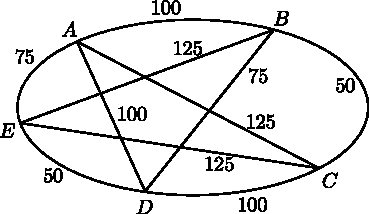
\includegraphics[scale=.8]{figures/ques-2.3.pdf}
		\caption{旅行商问题} \label{Fig:TSP-problem}
		\vspace{1cm}
				\begin{forest}
		  for tree={
		    draw,
		    circle,
		  },
		  [A
		  	[B, edge label={node[midway,left,font=\scriptsize]{100}}
		  		[C, edge label={node[midway,left,font=\scriptsize]{150}}
		  			[D, edge label={node[midway,left,font=\scriptsize]{100}}
		  				[E, edge label={node[midway,right,font=\scriptsize]{50}}
		  					[A, edge label={node[midway,right,font=\scriptsize]{75}}
		  					]]]
		  			[E, edge label={node[midway,right,font=\scriptsize]{125}}
		  				[D, edge label={node[midway,right,font=\scriptsize]{50}}
		  					[A, edge label={node[midway,right,font=\scriptsize]{100}}
		  					]]]
		  		][D, edge label={node[midway,right,font=\scriptsize]{75	}}
		  			[C, edge label={node[midway,left,font=\scriptsize]{100}}
		  				[E, edge label={node[midway,right,font=\scriptsize]{125}}
		  					[A, edge label={node[midway,right,font=\scriptsize]{75}}
		  					]]]
		  			[E, edge label={node[midway,right,font=\scriptsize]{50}}
		  				[C, edge label={node[midway,right,font=\scriptsize]{125}}
		  					[A, edge label={node[midway,right,font=\scriptsize]{125}}
		  					]]]
		  		][E, edge label={node[midway,right,font=\scriptsize]{125}}
					[C, edge label={node[midway,left,font=\scriptsize]{125}}
						[D, edge label={node[midway,right,font=\scriptsize]{100}}
							[A, edge label={node[midway,right,font=\scriptsize]{100}}
							]]]
					[D, edge label={node[midway,right,font=\scriptsize]{50}}
						[C, edge label={node[midway,right,font=\scriptsize]{100}}
							[A, edge label={node[midway,right,font=\scriptsize]{125}}
							]]]  		
		  		]
		  	][C][D][E]
		  ]
		\end{forest}
		\caption{旅行商问题状态空间图} \label{Fig:TSP-answer}
		\vspace{1cm}
		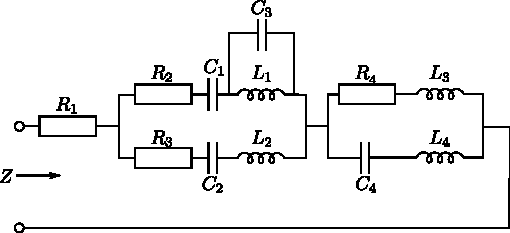
\includegraphics{figures/ques-2.4.pdf}
		\caption{电网络阻抗计算} \label{Fig:elec}
	\end{figure}
	
	\begin{figure}[H]
		\centering
		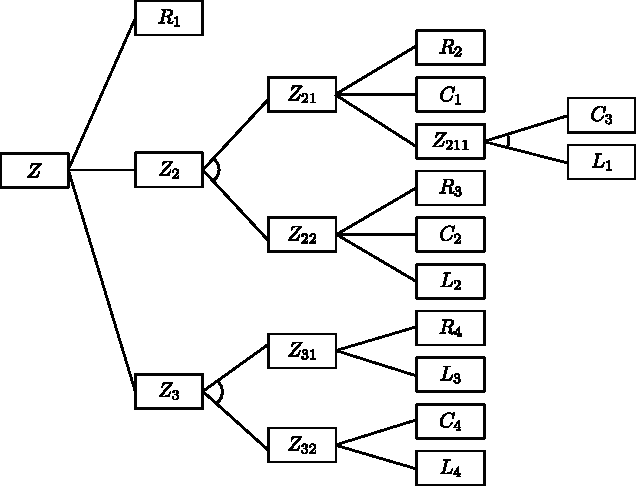
\includegraphics[scale=.8]{figures/ans-2.4.pdf}
		\caption{电网络阻抗计算与或解树} \label{Fig:and-or-tree-for-elec}
		\vspace{1cm}
		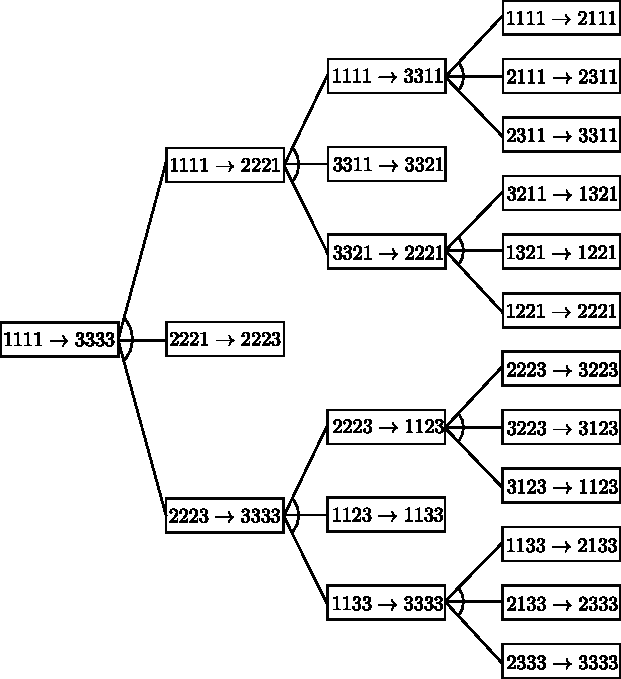
\includegraphics[scale=.8]{figures/ans-2.5.pdf}
		\caption{樊塔问题与或树} \label{Fig:and-or-tree-for-hannoi}
	\end{figure}

\begin{question}
把下列句子变换成子句形式:
	\begin{enumerate}
         \item $\left(\forall x\right) \left\{P\left(x\right) \to P\left(x\right)\right\}$
         \item $\forall x \forall y \left(\mathrm{On} \left(x,y\right) \to \mathrm{Above} \left(x,y\right) \right)$
         \item $\forall x \forall y \forall z \left(\mathrm{Above} \left(x,y\right) \wedge \mathrm{Above}\left(y,z\right) \to \mathrm{Above}\left(x,z\right) \right)$ 
         \item $\sim\left\{\left(\forall x\right)\left\{\left(\forall y)\left[p\left(y\right) \to p(f(x,y))\right] \wedge \left(\forall y \right) \left[Q(x,y) \to P(y) \right]\right\}\right\}\right\}$
	\end{enumerate}
\end{question}
\begin{solution}
	\begin{enumerate}
		\item $\sim P(x) \wedge P(x)$
		\item $\sim \mathrm{On}(x,y) \wedge \mathrm{Above}(x,y)$
		\item 
		\item 
	\end{enumerate}
\end{solution}

\begin{question}
用谓词演算公式表示下列英文句子(多用而不是省用不同谓词和项。例如不要用单一的谓词字母来表示每个句子)。
	\begin{quote}
		A computer system is intelligent if it can perform a task which, if performed by a human, requires intelligence. 
	\end{quote}
\end{question}
\begin{solution}
定义以下谓词:
	\begin{itemize}
		\item $\mathrm{INTLT}(x)$:	$x$ is intelligent.
		\item $\mathrm{PERFORM}(x,y)$:	$x$ can perform $y$.
		\item $\mathrm{REQUIRE}(x)$:		$x$ requires intelligence.
		\item $\mathrm{CMP}(x)$:		$x$ is a computer system.
		\item $\mathrm{HMN}(x)$:		$x$ is a human.
	\end{itemize} \par
则题中句子可以表达为
	\begin{multline*}
	\left( \exists t \right) \left( \exists y \right)
	\left[ \mathrm{HMN}(x) \vee \mathrm{PERFORM}(y,t) \vee \mathrm{REQUIRE}(t)
	\vee \mathrm{CMP}(x) \right. \\
	\left. \vee \mathrm{PERFORM}(x,t) \right] 
	\to \mathrm{INTLT}(x)
	\end{multline*}
\end{solution}

\begin{question}
把下列语句表示称语义网络描述:
	\begin{enumerate}
		\item All men are moral.
		\item Every cloud has a silver lining.
		\item All branch manager of DEC participate in a profit-sharing plan. 
	\end{enumerate}
\end{question}
\begin{solution}
如图\ref{Fig:semantic-net}。
	\begin{figure}[h]
		\centering
		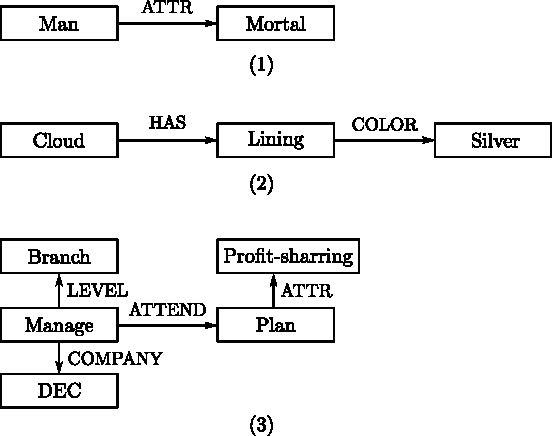
\includegraphics[scale=.9]{figures/ans-2.8.pdf}
		\caption{ 所求语义网络 } \label{Fig:semantic-net}
	\end{figure}
\end{solution}

\begin{question}
试构造一个描述你的寝室或办公室的框架系统。
\end{question}
\begin{solution}
以房间为例,如图\ref{Fig:semantic-my-room}。
	\begin{figure}[h]
		\centering
		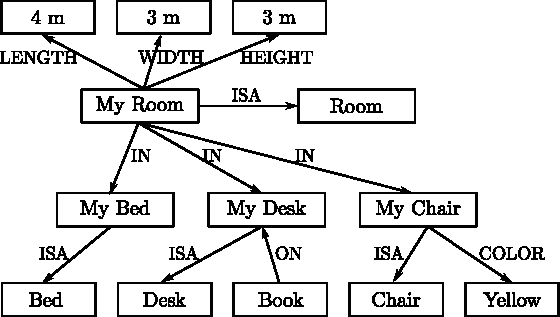
\includegraphics[scale=.9]{figures/ans-2.9.pdf}
		\caption{ 我的房间语义网络 } \label{Fig:semantic-my-room}
	\end{figure}
\end{solution}

\begin{question}
框架和本体有何关系与区别?
\end{question}
\begin{solution}
\end{solution}

\end{document}